\section{Modularization}

% -----------------------------------
\subsection{Modularization Motivation}

\begin{frame}
\frametitle{Why Modularization}
\begin{itemize}
\item Growth management
\pause
\item Software quality improvement
\pause
\item Facilitating add-ons
\pause
\item Separate third party libraries
\pause
\item Optional Components
\end{itemize}
\end{frame}

% -----------------------------------
\subsection{Modularization Implementation}

\begin{frame}
\frametitle{Module sizes}
\center
\begin{center}
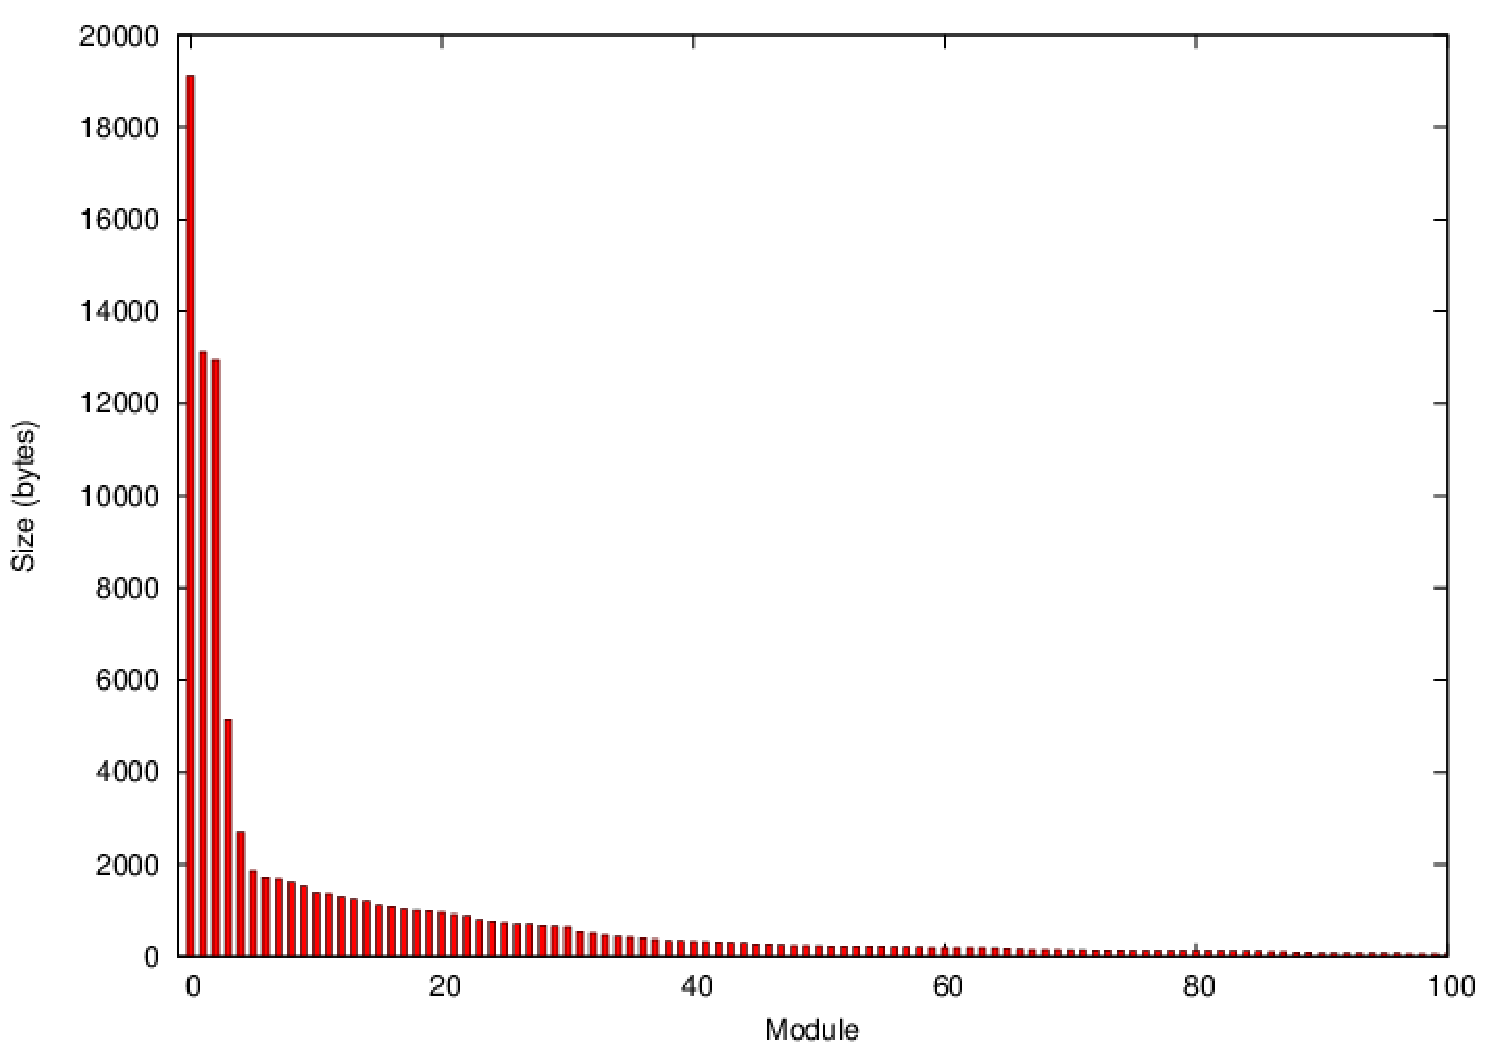
\includegraphics[height=0.8\textheight]{../Art/moduleSizePlot.pdf}
\end{center}
\end{frame}

\begin{frame}
\frametitle{Module sizes (no third party modules)}
\center
\begin{center}
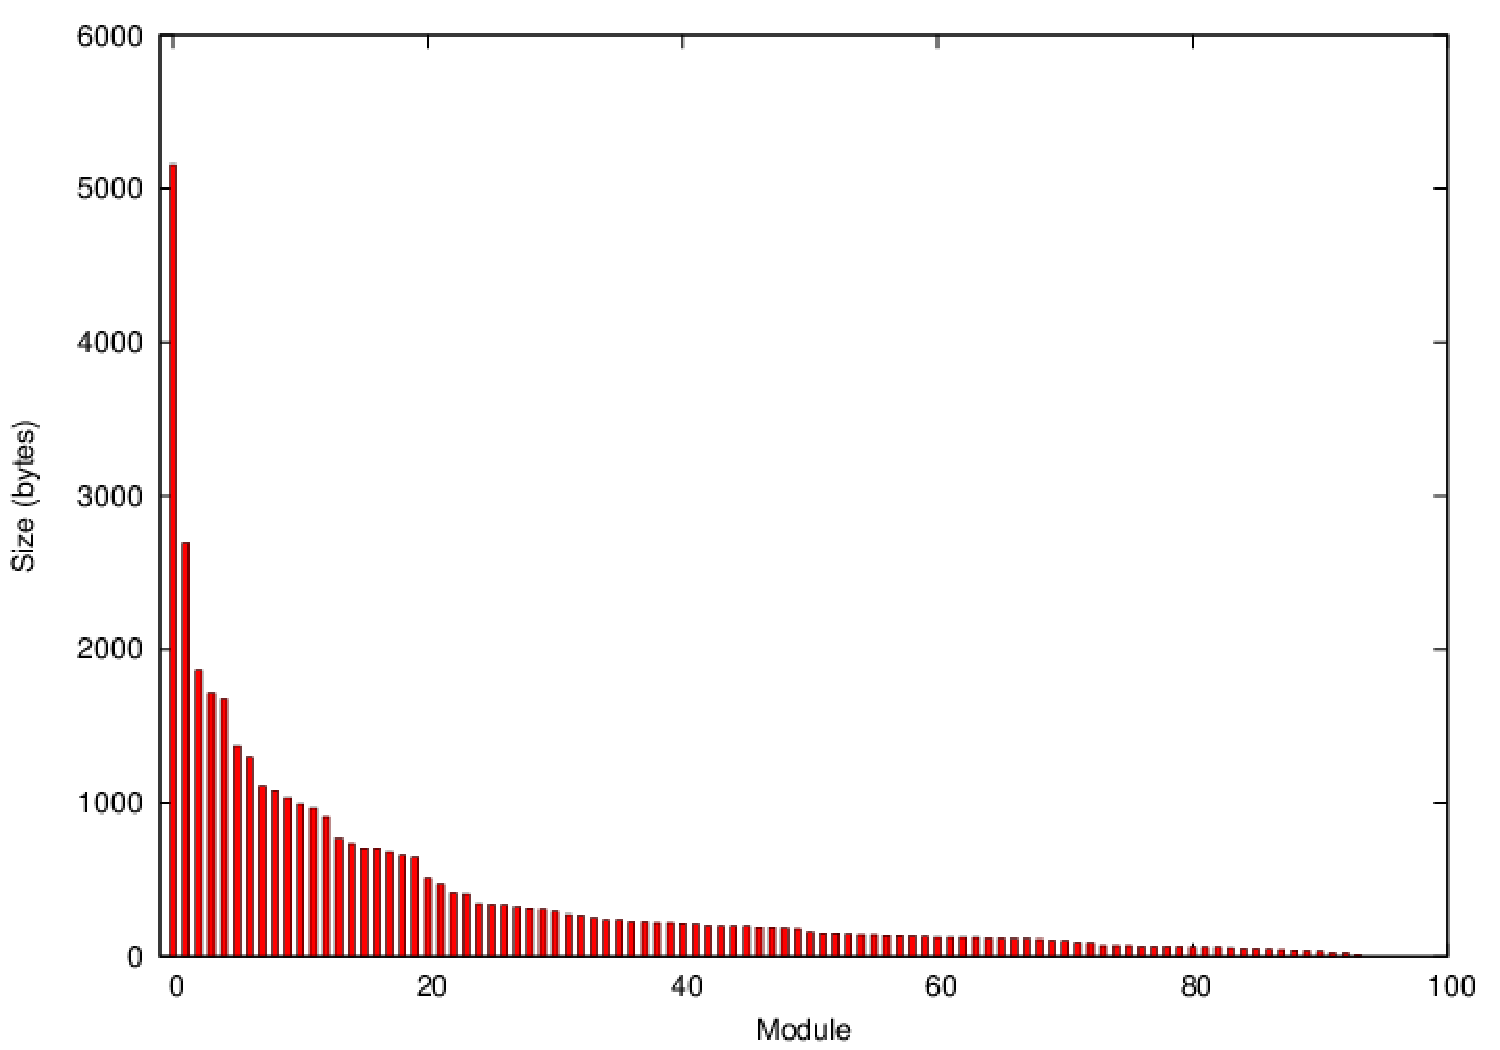
\includegraphics[height=0.8\textheight]{../Art/moduleSizePlotNoThirdParty.pdf}
\end{center}
\end{frame}

\begin{frame}
\frametitle{Visualize dependencies among modules}
\center
\begin{center}
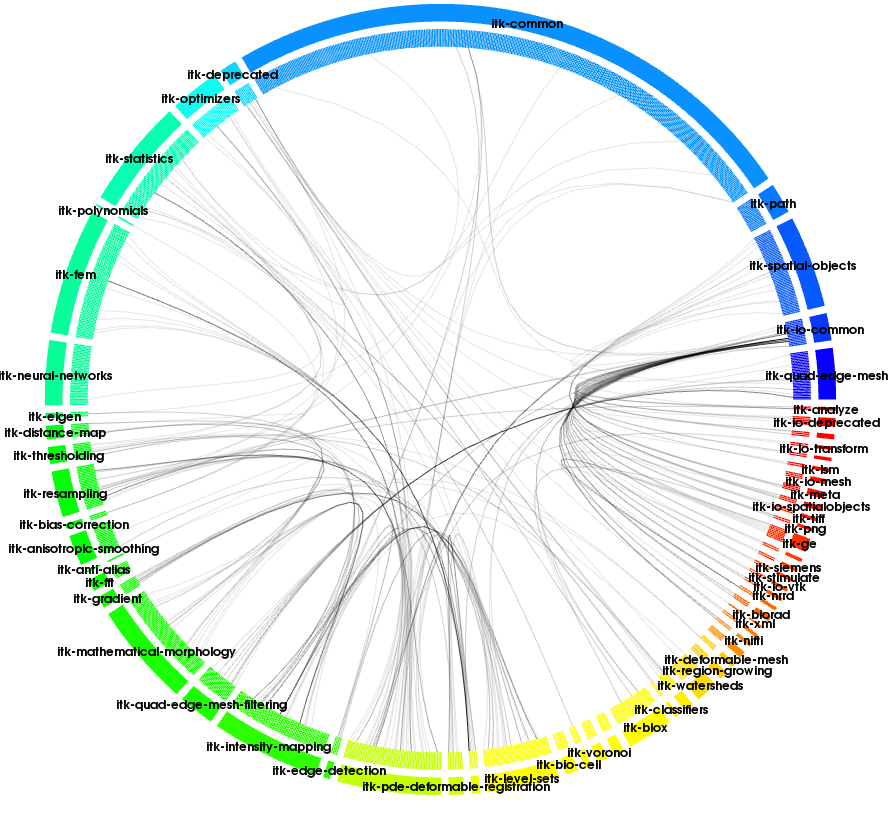
\includegraphics[height=0.8\textheight]{../Art/moduleDependency.png}
\end{center}
\end{frame}

\begin{frame}
\frametitle{ITK Module Grouping}
\begin{itemize}
\item  12 groups, 110 modules and counting
\pause
\item  Grouped by module functionality
\pause
\end{itemize}
\vskip14pt
%\begin{block}
\begin{tabular}{llll}
Bridge     &    \alert{External}   & IO        & Registration \\
Compatibility  & Filtering  & Nonunit   & Segmentation \\
Core           & GPU        & Numerics  & ThirdParty \\
\end{tabular}
%\end{block}
\end{frame}

% -----------------------------------
\subsection{Add Your Own Module}

\begin{frame}
\frametitle{How to add a module into ITK}
\begin{enumerate}
\item Decide where to put the module
\pause
\item Create the CMake setup
\pause
\item Add its content
\end{enumerate}
\end{frame}


\begin{frame}[fragile]
\frametitle{Modularization checklist}
\begin{itemize}
\item<1->\textbf{Module categorization}: \alt<1,4->{module group, module name}{
\begin{itemize}
\item<2-> Group is specified by the directory
\item<3-> Module name is specified by directory, \texttt{itk-module.cmake}
\end{itemize}
}
\item<4->\textbf{Directory hierarchy}: \alt<4,8->{\texttt{include},\textcolor{gray}{\texttt{src}}, \texttt{test}}{
\begin{itemize}
\item<5-> \textbf{include}: Headers defining the API, \texttt{*.hxx} template implementations
\item<6-> \textcolor{gray}{\textbf{src}:  \texttt{*.cxx}  implementations, create a library}
\item<7-> \textbf{test}: Module unit tests
\end{itemize}
}
\item<8->\textbf{CMakeLists.txt} \alt<8,12->{top of module, \textcolor{gray}{\texttt{src}}, \texttt{test}}{
\begin{itemize}
\item<9-> \textbf{top of module}: \texttt{project()}, \texttt{itk\_module\_impl()}, \textcolor{gray}{\texttt{set(ITKFoo\_LIBRARIES ITKFoo)}}
\item<10-> \textcolor{gray}{\textbf{src}: \texttt{add\_library()}, \texttt{target\_link\_library()},\texttt{itk\_module\_target()}}
\item<11-> \textbf{test}: \texttt{itk\_module\_test()}, \texttt{itk\_add\_test()}
\end{itemize}
}
\item<12->\textbf{Module dependencies and documentation} \texttt{itk-module.cmake}
\end{itemize}
\end{frame}


% -----------------------------------
\subsection{Exercise}
\begin{frame}
\frametitle{Exercise: ITKRAT}
\small
\begin{itemize}
\item  Insight Journal article on itkRobustAutomaticThresholdImageFilter(RAT)
\item
\texttt{~/src/ITKv4-TheNextGenerationTutorial/}\\
\texttt{Exercises/Modularization/IJ-submission-rat}
\item  Make into an External module: ITKRAT
\end{itemize}
\end{frame}


\begin{frame}
\frametitle{More information on modularization}
\begin{itemize}
\item  Details about ITK Modularization can be found at \href{http://www.itk.org/Wiki/ITK\_Release\_4/Modularization}{\textcolor{red}{\underline{Wiki Page}}}.
\end{itemize}
\end{frame}
